%%% template.tex
%%%
%%% This LaTeX source document can be used as the basis for your technical
%%% paper or abstract.

%%% The parameter to the ``documentclass'' command is very important.
%%% - use ``review'' for content submitted for review.
%%% - use ``preprint'' for accepted content you are making available.
%%% - use ``tog'' for technical papers accepted to the TOG journal and
%%%   for presentation at the SIGGRAPH or SIGGRAPH Asia conference.
%%% - use ``conference'' for final content accepted to a sponsored event
%%%   (hint: If you don't know, you should use ``conference.'')

\documentclass[conference]{acmsiggraph}

%%% Make the ``BibTeX'' word pretty...

\def\BibTeX{{\rm B\kern-.05em{\sc i\kern-.025em b}\kern-.08em
    T\kern-.1667em\lower.7ex\hbox{E}\kern-.125emX}}

\title{Real Time NeuroEvolution of Augmenting Topologies in video games}

%%% TODO: Mettre les adresses de l'école
\author{Guillaume Ambrois\thanks{e-mail:guillaume.ambrois@gmail.com}, Sébastien Gaulier\thanks{e-mail:sebastien.gaulier@gmail.com}\\ESGI, Paris}
\pdfauthor{Guillaume Ambrois & Sébastien Gaulier}

%%% TODO: Ajouter des mots clés
\keywords{video game, artificial intelligence, machine learning, NeuroEvolution of Augmenting Topologies}

\begin{document}

%%% This is the ``teaser'' command, which puts an figure, centered, below 
%%% the title and author information, and above the body of the content.

%%% TODO: Changer l'image
 \teaser{
   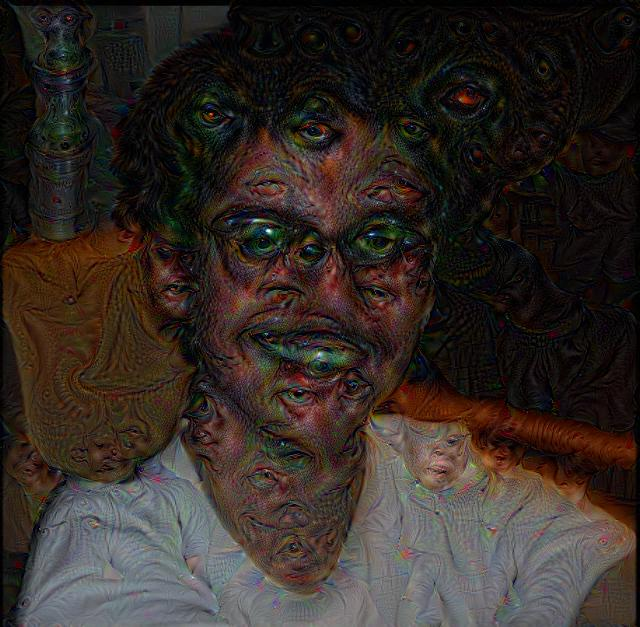
\includegraphics[height=1.5in]{images/sampleteaser}
   \caption{NERO, showcase video game for rtNEAT}
 }

\maketitle

\begin{abstract}

Artificial Intelligence is one of the fields that advances the most in video games, but there is still a tremendous work to be done.

In this poster, we will talk about how we can achieve real time Machine Learning, using rtNEAT.

\end{abstract}

\keywordlist

%% Required for all content. 

\copyrightspace

\section{Introduction}

Plein de texte pour pousser les références.
Plein de texte pour pousser les références.
Plein de texte pour pousser les références.
Plein de texte pour pousser les références.
Plein de texte pour pousser les références.
Plein de texte pour pousser les références.
Plein de texte pour pousser les références.
Plein de texte pour pousser les références.
Plein de texte pour pousser les références.

\section{Using rtNEAT}

La bibliothèque rtNEAT est une implémentation temps réel en C++ de la méthode de NeuroEvolution of Augmenting Topologies.

Plein de texte pour pousser les références.
Plein de texte pour pousser les références.
Plein de texte pour pousser les références.
Plein de texte pour pousser les références.
Plein de texte pour pousser les références.
Plein de texte pour pousser les références.
Plein de texte pour pousser les références.
Plein de texte pour pousser les références.
Plein de texte pour pousser les références.
Plein de texte pour pousser les références.
Plein de texte pour pousser les références.
Plein de texte pour pousser les références.
Plein de texte pour pousser les références.
Plein de texte pour pousser les références.
Plein de texte pour pousser les références.
Plein de texte pour pousser les références.

\section{Our approach}

Plein de texte pour pousser les références.
Plein de texte pour pousser les références.
Plein de texte pour pousser les références.
Plein de texte pour pousser les références.
Plein de texte pour pousser les références.
Plein de texte pour pousser les références.
Plein de texte pour pousser les références.
Plein de texte pour pousser les références.
Plein de texte pour pousser les références.
Plein de texte pour pousser les références.
Plein de texte pour pousser les références.
Plein de texte pour pousser les références.
Plein de texte pour pousser les références.
Plein de texte pour pousser les références.
Plein de texte pour pousser les références.
Plein de texte pour pousser les références.
Plein de texte pour pousser les références.
Plein de texte pour pousser les références.
Plein de texte pour pousser les références.
Plein de texte pour pousser les références.
Plein de texte pour pousser les références.
Plein de texte pour pousser les références.
Plein de texte pour pousser les références.
Plein de texte pour pousser les références.
Plein de texte pour pousser les références.
Plein de texte pour pousser les références.
Plein de texte pour pousser les références.
Plein de texte pour pousser les références.
Plein de texte pour pousser les références.

\bibliographystyle{acmsiggraph}
\nocite{*}
\bibliography{template}
\end{document}
